\documentclass[10pt,a4paper]{article}
\usepackage[utf8]{inputenc}
\usepackage[english]{babel}
\usepackage{amsmath}
\usepackage{amsfonts}
\usepackage{amssymb}
\usepackage{makeidx}
\usepackage{graphicx}
\usepackage{lmodern}
\usepackage{bm}
\usepackage{tikz}
\usepackage{amsthm}
\usetikzlibrary{calc}
\usepackage[left=2cm,right=2cm,top=2cm,bottom=2cm]{geometry}
\author{Djordje Zivanovic}
\title{\textbf{Warsaw PhD Open Course: From Joins to Aggregates and
Optimization Problems - Exam solutions}}
\begin{document}
\maketitle
\bigskip
%Chapter 1 in Ockendon \& Tayler: Applied PDE's  
%{\it Maths Institute Lecture Notes}. 	
%{\bf Exercises 1, 2, 4, 5}.
\newcommand{\transpose}[1]{#1 ^ \text{T}}
\newcommand{\mat}[1]{\textbf{\text{{#1}}}}
\newcommand{\vect}[1]{\mat{#1}}
\newcommand{\gradient}[1]{\nabla_{\vect{#1}}}
\newcommand{\der}[1]{\frac{\partial}{\partial #1}}
\newcommand{\numberthis}{\addtocounter{equation}{1}\tag{\theequation}}
\newcommand{\logfun}{\sigma(\transpose{\vect{x}}_i \vect{w})}
\newcommand{\softmaxi}{\frac{e^{z_i}}{\sum_{l=1}^Ce^{z_l}}}
\newcommand{\layersep}{2.5cm}
\newcommand{\layersepH}{6cm}
\newcommand{\layersepP}{7cm}
\newcommand{\layersepB}{9cm}
\newtheorem{theorem}{Theorem}
\newtheorem{lemma}[theorem]{Lemma}
\begin{enumerate}
\item[1]
Let $Q(\mathbf{A_1} \cup \mathbf{A_2} \cup \cdots \cup \mathbf{A_n})$ denote a join query on relations $R_1(\mathbf{A_1})=R_1(A_1, A_2), \cdots R_n(\mathbf{A_n})=R_n(A_n, A_1)$.

Let $\mathcal{H}=(\mathcal{V}, \mathcal{E})$ denote a corresponding hypegraph to the join query, then $\mathcal{V} = \{A_1, .., A_n\}$ and $\mathcal{E} =\{\{A_1, A_2\}, ..., \{A_n, A_1\}\}$.
\begin{enumerate}
\item[1.1]
Let $x_{R_i}$ denote the weight of an hyperedge (relation) $R_i$ in the join query $Q$. In addition let $cover_i$ denote the set of relations corresponding to edges that are part of the cover for the variable $i$. The fractional edge cover number $\rho^{*}(Q)$ is the cost of an optimal solution to the linear program:
\begin{eqnarray}
\text{minimize} \sum_{i\in [n]} x_{R_i}  \label{eq:minimize} \\
\text{subject to} \sum_{rel_j \in cover_i} x_{rel_j} \geq 1, i \in [n]  \label{eq:inequalities}\\
x_{R_i} \geq 0, i \in [n] \nonumber
\end{eqnarray}

By a definition of a cover, only edges incident  to variable are part of its cover. Thus, in our case $cover_i =\{ R_{i-1}, R_i \}$, where $R_0$ is $R_n$ in the case of $A_1$. If we rewrite the inequalities \ref{eq:inequalities} we will get:
\begin{eqnarray}
x_{R_1} +  x_{R_n} \geq 1 \nonumber \\
x_{R_1} +  x_{R_2} \geq 1\nonumber \\
\vdots \nonumber \\
x_{R_{n-1}} +  x_{R_n} \geq 1 \nonumber
\end{eqnarray}
By summing inequalities we get:
$$2\left(\sum_{i\in [n]} x_{R_i}\right) \geq n$$
\end{enumerate}
This means the minimized function $\rho^*(Q)$ cannot  be less than $\frac{n}{2}$. This is achievable if we set $x_{R_i}=\frac{1}{2}, i \in [n]$. We can see that this solution satisfies all constraints in the linear program. Finally, $\rho^*(Q)=\frac{n}{2}$. 
\\
A width of a specific hypertree decomposition is defined as a maximum among all edge covers for each of the nodes of the hypertree. A hypertree width (htw) for the specific query Q is defined as a minimum width among all possible widths of hypertree decompositions of a query Q. 
\\
A fractional width of a specific hypertree decomposition is defined as a maximum among all fractional edge covers for each of the nodes of the hypertree. A fractional hypertree width (fhtw) for the specific query Q is defined as a minimum width among all possible widths of hypertree decompositions of a query Q.
The only difference is that in the case of fractional hypertree width we use fractional edge covers instead of edge covers. \\
In the case of $n=2$ $fhtw(Q) = htw(Q) = 1$. For $n >= 3$ the hypertree decomposition on the figure \ref{fig:fthw} is the optimal one. From picture we can figure out that $htw(Q)=2$ in all cases, while $fhtw(Q)=2$ for $n>3$, but for $n=3$ it is $\frac{3}{2}$. 
\\
The decomposition on the figure \ref{fig:fthw} is optimal because we have to "propagate" one variable through nodes of the hypertree in order to fulfill the condition that all hyperedges of hypergraph are contained in the nodes of hypertree. Adding more than three variables inside a node of hypertree would increase (fractional) width of a hypertree decomoposition because we would need to cover at least two variables that are not in the same relation.  (Fractional) edge cover number for each of nodes of hypegraph inside nodes of hyperetree is $2$ because $A_1 A_iA_{i-1}$ can be covered with $x_{R_i}=1, x_{R_1}=1$. The only exception to the previous case is $n=3$ where fractional edge cover of $\frac{3}{2}$ is possible. 
\begin{figure}
\begin{center}
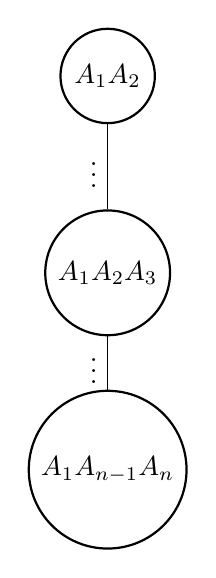
\begin{tikzpicture}
\begin{scope}[every node/.style={circle,thick,draw}]
    \node (C) at (2.5,2.5) {$A_1 A_2$};
    \node (D) at (2.5,0) {$A_1 A_2 A_3$};
    \node (E) at (2.5,-2.5) {$A_1 A_{n-1}A_{n}$};
\end{scope}
\begin{scope}
    \path  (C) edge node {$\vdots$    \, \,} (D);
    \path[]  (D) edge node {$\vdots$    \, \,} (E);
\end{scope}
\end{tikzpicture} 
\end{center}
\caption{Hypertree decomposition that corresponds to fhtw}
\label{fig:fthw}
\end{figure}

\item[1.2]
A size of listing representation is $\mathcal{O}(N^{\rho^*(Q)})=\mathcal{O}(N^{\frac{n}{2}})$ and can be computed in time $\mathcal{O}(N^{\rho^*(Q)})=\mathcal{O}(N^{\frac{n}{2}})$.
A loss function is:
\begin{eqnarray}
2|D|\mathcal{L}(\mat{X},\vect{y}, \mathbf{\theta})  &=& (\vect{y} - \mat{X}\mathbf{\theta})^2 \nonumber + \lambda ||\mathbf{\theta}||_2^2\\
			&=& \transpose{(\vect{y} - \mat{X}\mathbf{\theta})}(\vect{y} - \mat{X}\mathbf{\theta}) + \lambda ||\mathbf{\theta}||_2^2 \nonumber \\
&=&\transpose{\vect{y}}\vect{y} - \transpose{\vect{y}}\mat{X}\mathbf{\theta}
- \transpose{\mathbf{\theta}}\transpose{\mat{X}} \vect{y}
+ \transpose{\mathbf{\theta}}\transpose{\mat{X}}\mat{X}\mathbf{\theta} + \lambda ||\mathbf{\theta}||_2^2 \nonumber \\
&=&
\transpose{\vect{y}}\vect{y} - 2 \transpose{\vect{y}}\mat{X}\mathbf{\theta}
+ \transpose{\mathbf{\theta}}\transpose{\mat{X}}\mat{X}\mathbf{\theta} + \lambda\transpose{\mathbf{\theta}}\mathbf{\theta}
\label{eq:loss}
\end{eqnarray}
In the equation \ref{eq:loss} we used the property that transpose of a scalar is the same scalar. All equations before that are simple vector multiplications and additions. 
If we derive the equation \ref{eq:loss} we get the gradient of the loss function: :
\begin{eqnarray}
\nabla_{\mathbf{\theta}} \mathcal{L}(\mat{X},\vect{y}, \mathbf{\theta}) &=& 0  - \frac{1}{|D|}\transpose{\mat{X}}\vect{y} + \frac{1}{|D|}\transpose{\mat{X}}\mat{X}\mathbf{\theta} + \lambda \frac{1}{|D|}\mathbf{\theta} \nonumber \\
&=& \frac{1}{|D|}\transpose{\mat{X}}\mat{X}\mathbf{\theta} - \frac{1}{|D|}\transpose{\mat{X}}\vect{y} + \lambda\frac{1}{|D|}\mathbf{\theta}\nonumber
\end{eqnarray}
A gradient descent formula is:
$$\mathbf{\theta}_{t+1}=\mathbf{\theta}_t - \eta\nabla_{\mathbf{\theta}} \mathcal{L}(\mat{X},\vect{y}, \mathbf{\theta})$$
After joining relations we need in each step to calculate gradient. 
We can notice that $\transpose{\mat{X}}\vect{y}$ can be cached and the complexity to do so is $\mathcal{O}(n \cdot N^\frac{n}{2})$. Similarly with $\transpose{\mat{X}}\mat{X}$, whose calculation takes $\mathcal{O}(n^2 \cdot N^\frac{n}{2})$. In each iteration we need to multiply $\transpose{\mat{X}}\mat{X}$ with $\mathbf{\theta}$ which takes $\mathcal{O}(n^2)$ time.  
When we add  all time complexities we get:
$$\mathcal{O}(N^\frac{n}{2} + n^2 \cdot N^\frac{n}{2} + n \cdot  N^\frac{n}{2} + n^2 \cdot t) $$

Memory complexity after the join is
$\mathcal{O}(N^\frac{n}{2})$. $\transpose{\mat{X}}\mat{X}$ cached takes $\mathcal{O}(n^2)$ and $\transpose{\mat{X}}\vect{y}$ takes $\mathcal{O}(n)$.
When we add these complexities we get memory complexity at each iteration is:
$\mathcal{O}(n^2)$. 


\end{enumerate}

\end{document}